\documentclass[10pt,a4paper]{article}
\usepackage[margin=1.7cm]{geometry}
\usepackage{graphicx}
\usepackage{booktabs}
\usepackage{microtype}
\usepackage{caption}
\usepackage{subcaption}
\usepackage{amsmath}
\usepackage{amssymb}
\usepackage{url}
\usepackage{xcolor}
\usepackage[hidelinks]{hyperref}
\usepackage[round,authoryear]{natbib}
\usepackage{titlesec}
\usepackage{enumitem}

% -- Typography & layout -------------------------------------------------------
\definecolor{accent}{HTML}{1F3A5F}
\titlespacing*{\section}{0pt}{1.0ex}{0.4ex}
\titlespacing*{\subsection}{0pt}{0.5ex}{0.2ex}
\titleformat{\section}{\normalsize\bfseries\color{accent}}{\thesection}{0.6em}{}
\titleformat{\subsection}{\small\bfseries}{\thesubsection}{0.5em}{}
\setlength{\parskip}{2.5pt}
\setlength{\parindent}{0pt}
\renewcommand{\arraystretch}{1.10}
\captionsetup{font=footnotesize,labelfont={bf,color=accent},skip=2pt}
\captionsetup[sub]{font=footnotesize,labelfont=bf,skip=1pt}
\setlist{nosep,leftmargin=*}
\pagestyle{empty}

\begin{document}

% -- Title block ---------------------------------------------------------------
\begingroup
\centering
{\Large\bfseries\color{accent} Calibrated Uncertainty under Image Perturbations\\for Galaxy Morphology Classification\par}
\vspace{3pt}
{\small COMP90051 Statistical Machine Learning \textbar{} 2026 Semester 1 Group Project}\\
{\small Student IDs: [REDACTED FOR SUBMISSION]}\par
\vspace{2pt}
{\color{accent}\rule{\linewidth}{0.6pt}}
\endgroup
\vspace{-4pt}

% -- Introduction --------------------------------------------------------------
\section{Introduction}
\textbf{Research question.} Galaxy morphology classifiers will eventually be applied to images that differ from their training distribution -- atmospheric blur, instrumental noise, cosmic-ray hits that occlude pixels, and arbitrary sky-plane rotations are all unavoidable. Beyond predictive accuracy we therefore ask: \textbf{how does the predictive calibration of three classifiers of increasing complexity degrade as test images are progressively corrupted, and is a model's clean-data calibration ranking preserved under shift?} This goes beyond ``predict the class'' (the obvious dataset task) and beyond a head-to-head accuracy comparison: the central artefact is a calibration-vs-perturbation curve for each model. The motivation is operational -- a downstream science pipeline that consumes class probabilities (e.g.\ to weight likelihoods in a population study) needs to know when those probabilities can be trusted, not merely how often the top-1 label is right.

\textbf{Dataset.} Galaxy10 DECaLS\footnote{\url{https://astronn.readthedocs.io/en/latest/galaxy10.html}} (Leung \& Bovy, 2019): $17{,}736$ DECaLS RGB cutouts at $256\!\times\!256$\,px with 10 morphology classes (Disturbed, Merging, Round Smooth, In-between Round Smooth, Cigar Shaped Smooth, Barred Spiral, Unbarred Tight Spiral, Unbarred Loose Spiral, Edge-on without Bulge, Edge-on with Bulge). The dataset is moderately imbalanced (Cigar: $n{=}334$; Round Smooth: $n{=}2{,}645$), satisfying the $\geq\!10{,}000$ images and $\geq\!100{\times}100$\,px requirement.

% -- Literature ----------------------------------------------------------------
\section{Literature review}
The dataset itself is from astroNN \citep{leung2019}, who curated DECaLS cutouts using Galaxy Zoo morphology votes. Galaxy Zoo crowdsourcing \citep{lintott2008} and the original morphological taxonomy frame what a ``correct'' label means. \citet{dieleman2015} introduced CNNs with rotational averaging to galaxy morphology, establishing the modern baseline. The post-2016 research-paper algorithm we implement is the deep-ensembles framework of \citet{lakshminarayanan2017} (NeurIPS 2017, not covered in class), which trains $M$ independent networks from different initialisations and averages their softmax outputs, yielding better-calibrated predictions than a single network. The two papers closest to our research question are \citet{ovadia2019} (NeurIPS 2019), who systematically show that no single uncertainty method retains its clean-data calibration ranking under distribution shift, and \citet{hendrycks2019} (ICLR 2019), whose ImageNet-C corruption framework directly motivates our four perturbation families. Calibration metrics follow \citet{guo2017}; the CAS and Gini--$M_{20}$ morphology indicators we use as features are from \citet{conselice2003} and \citet{lotz2004}.

% -- Methods -------------------------------------------------------------------
\section{Methods}
\subsection{Feature construction and preprocessing (\S 2.c)}
Image inputs are decoded to \texttt{float32}\,$\in[0,1]$ and, for the CNN, downsampled to $64\!\times\!64$ (the perturbation sweep uses $32\!\times\!32$ to keep the 20-condition cartesian grid tractable). Per-fold standardisation is fit on the training partition only. Augmentation -- per-sample horizontal flip and uniform $\{0^\circ,90^\circ,180^\circ,270^\circ\}$ rotation drawn independently per sample in each mini-batch -- is applied to training images only; galaxies have no canonical orientation so multiples of $90^\circ$ are exact label-preserving transformations.

Handcrafted features for the LR and RF models are 113 numbers per image (\(>\!100\) as required) split into six groups: (i)~\textbf{photometric} (16): mean/std/skew/kurtosis of R, G, B and grayscale channels; (ii)~\textbf{CAS+Gini--$M_{20}$} (10): concentration, asymmetry, smoothness, Gini, $M_{20}$, ellipticity, orientation, Sersic-like concentration, half-light and Petrosian radii, all evaluated within $1.5\!\times\!r_{\text{Pet}}$ after corner-based sky subtraction; (iii)~\textbf{radial} (20): 10-bin grayscale and 10-bin (G$-$R) colour-ratio radial profiles; (iv)~\textbf{Hu invariants} (7): log-transformed Hu moments; (v)~\textbf{HOG} (36): 2$\times$2 cell, 9-orientation descriptor; (vi)~\textbf{Gabor} (24): mean and std of the magnitude response of a 3-frequency $\times$ 4-orientation filter bank, convolved via FFT.

\subsection{Three classifiers of different complexity (\S 2.d)}
\textbf{Simple -- Multinomial Logistic Regression (from scratch).} Pure-NumPy softmax regression with L2 regularisation, fit by full-batch gradient descent; sklearn's $C$ semantics are mirrored with a $1/N$-normalised penalty gradient so that selected $C$ values are comparable to references.\\
\textbf{Medium -- Random Forest.} Sklearn \texttt{RandomForestClassifier} (\texttt{n\_jobs=-1}, \texttt{class\_weight="balanced"}) on the same 113 features.\\
\textbf{Complex -- Deep Ensemble CNN \citep{lakshminarayanan2017}.} Five independent four-block VGG-style CNNs (Conv-BN-ReLU $\rightarrow$ Pool $\times 3$, then $128\!\times\!2\!\times\!2$ adaptive pool $\rightarrow$ dropout-MLP) trained with AdamW + class-weighted cross-entropy and a 10\% stratified hold-out for early stopping (patience 5, max 20 epochs). The ensemble probability is the mean of the per-member softmaxes, which lets us additionally decompose the total predictive entropy into an aleatoric component (mean per-member entropy) and an epistemic component (Jensen gap between the entropy of the mean and the mean of the entropies).

\subsection{Cross-validation, hyperparameter tuning and metrics (\S 2.e--g)}
\textbf{Nested CV, implemented from scratch} (\texttt{src/galaxy\_uq/cv.py}): outer 10-fold stratified split (per-fold test size $\approx\!1{,}774$); inner 3-fold stratified split inside each outer training partition for HP selection; standardisation refit on each inner training partition to avoid test leakage. Folds are built by per-class \texttt{np.array\_split} after a seeded shuffle, with a final coverage assertion that every sample appears in exactly one outer test fold. The selection criterion is \textbf{macro-F1} -- the Cigar class is $<2\%$ of the data, so accuracy would be dominated by majority classes.

\textbf{Hyperparameter grids and tuning behaviour} (Tab.~\ref{tab:hps}). LR picks $C{=}10$ in 6/10 outer folds (middle of $\{0.1,1,10,100,10^3\}$); RF picks $\max_d{=}20$ in 6/10 folds (middle of $\{10,20,50\}$); CNN picks $\texttt{lr}{=}10^{-3}$ in 4/10 with neighbour $3{\cdot}10^{-4}$ in 4/10 and the extreme $3{\cdot}10^{-3}$ only 2/10, so 80\% of selections sit at the centre or one step away. The RF $n_{\text{est}}$ axis saturates at the top of an already once-extended grid ($\{200,500,1000\}\!\to\!\{500,1000,2000\}$, modal pick still the top): a structural property of bagging (variance reduction is monotone in tree count, bias unchanged), not an under-explored hyperparameter -- so we accept the boundary rather than pushing CV beyond tractable. HP-selection plots (Figs.~\texttt{03/04/05\_*\_hp\_selection.png}) show the inner macro-F1 surface is bowl-shaped in $C$, $\max_d$ and \texttt{lr}.

\textbf{Metrics, all implemented from scratch} (\texttt{src/galaxy\_uq/metrics.py}): accuracy, macro-F1 (mean of per-class F1 from a from-scratch confusion matrix), \textbf{Expected Calibration Error} (15 equal-width bins on max-softmax confidence, weighted absolute confidence--accuracy gap; \citealp{guo2017}), and \textbf{NLL} (mean per-sample negative log-likelihood of the true class, clipped to $[10^{-12},1{-}10^{-12}]$). Reliability bins are reported with NaN-safe per-bin accuracy. All reported error bars are $\pm 1\sigma$ across the ten outer folds.

\textbf{Perturbation protocol (the research question).} We re-train a CNN on outer-fold-0 train data with the modal HP and evaluate it on the same held-out test set under four corruption families: Gaussian blur ($\sigma\!\in\!\{0,1,2,4,8\}$\,px), additive Gaussian pixel noise ($\sigma\!\in\!\{0,10,25,50,100\}$ on the 0--255 scale), centred square occlusion ($s\!\in\!\{0,32,64,96,128\}$\,px), and rotation ($\theta\!\in\!\{0^\circ,15^\circ,45^\circ,90^\circ,180^\circ\}$). LR and RF baselines are evaluated on the same hold-out for context. This sweep uses a smaller CNN ($32\!\times\!32$, $M{=}2$, 5 epochs) to keep the 20-condition matrix tractable; the absolute accuracies are therefore lower than the full ensemble (Tab.~\ref{tab:agg}), but the trend across corruption strength is the quantity of interest.

% -- Results -------------------------------------------------------------------
\section{Results and Discussion}

\begin{table}[h]
\centering\footnotesize
\setlength{\tabcolsep}{6pt}
\begin{tabular}{lcccc}
\toprule
Model & Accuracy & Macro-F1 & ECE & NLL \\
\midrule
LR (113 hand-crafted features) & $0.494\pm 0.013$ & $0.428\pm 0.011$ & $\mathbf{0.066\pm 0.011}$ & $1.468\pm 0.017$ \\
RF (113 hand-crafted features) & $0.511\pm 0.017$ & $0.460\pm 0.008$ & $0.139\pm 0.011$ & $1.457\pm 0.034$ \\
Deep Ensemble CNN ($M{=}5$, $64{\times}64$) & $\mathbf{0.604\pm 0.019}$ & $\mathbf{0.580\pm 0.019}$ & $0.137\pm 0.016$ & $\mathbf{1.175\pm 0.055}$ \\
\bottomrule
\end{tabular}
\caption{Nested $10\!\times\!3$ stratified CV. Mean $\pm$ std across 10 outer folds; best per column in bold.}\label{tab:agg}
\end{table}

\begin{table}[h]
\centering\footnotesize
\setlength{\tabcolsep}{6pt}
\begin{tabular}{lll}
\toprule
Model & Grid & Modal pick (10 folds) \\
\midrule
LR & $C\!\in\!\{0.1,1,10,100,1000\}$ & $C{=}10$ (6/10), $C{=}1$ (4/10) \\
RF & $n_{\text{est}}\!\in\!\{500,1000,2000\}$, $\max_d\!\in\!\{10,20,50\}$ & $\max_d{=}20$ (6/10), $n_{\text{est}}{=}2000$ (7/10)$^\dagger$ \\
CNN & $\text{lr}\!\in\!\{3{\cdot}10^{-4},10^{-3},3{\cdot}10^{-3}\}$ & $\text{lr}{=}10^{-3}$ (4/10), $3{\cdot}10^{-4}$ (4/10) \\
\bottomrule
\end{tabular}
\caption{Hyperparameter grids (\S 2.f). $^\dagger$ RF $n_{\text{est}}$ saturates: a property of bagging, not an under-explored grid (see text).}\label{tab:hps}
\end{table}

\begin{figure}[h]
\centering
\begin{subfigure}{0.49\textwidth}
  
\includegraphics[width=\linewidth]{../results/figures/05b_reliability_comparison.png}
  \caption{Reliability diagrams.}
\end{subfigure}\hfill
\begin{subfigure}{0.49\textwidth}
  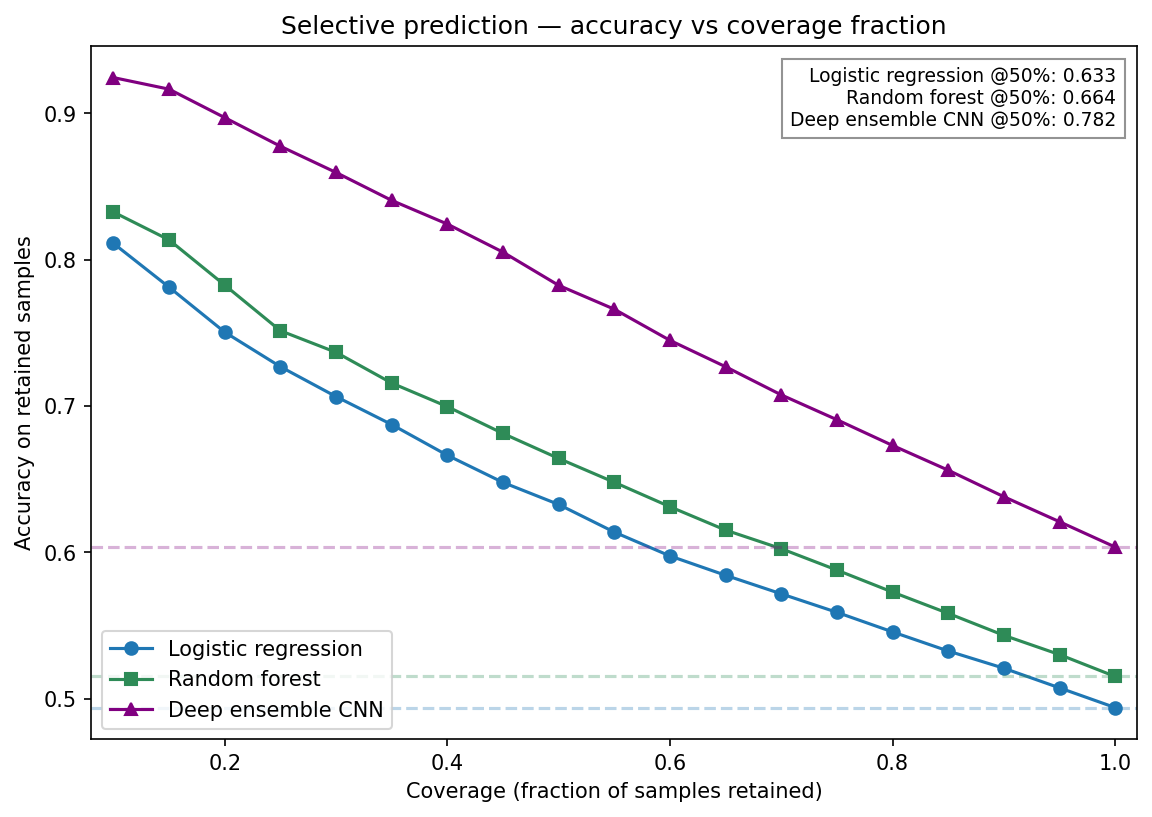
\includegraphics[width=\linewidth]{../results/figures/05b_risk_coverage.png}
  \caption{Risk--coverage on CNN max-softmax.}
\end{subfigure}\\[4pt]
\begin{subfigure}{0.92\textwidth}
  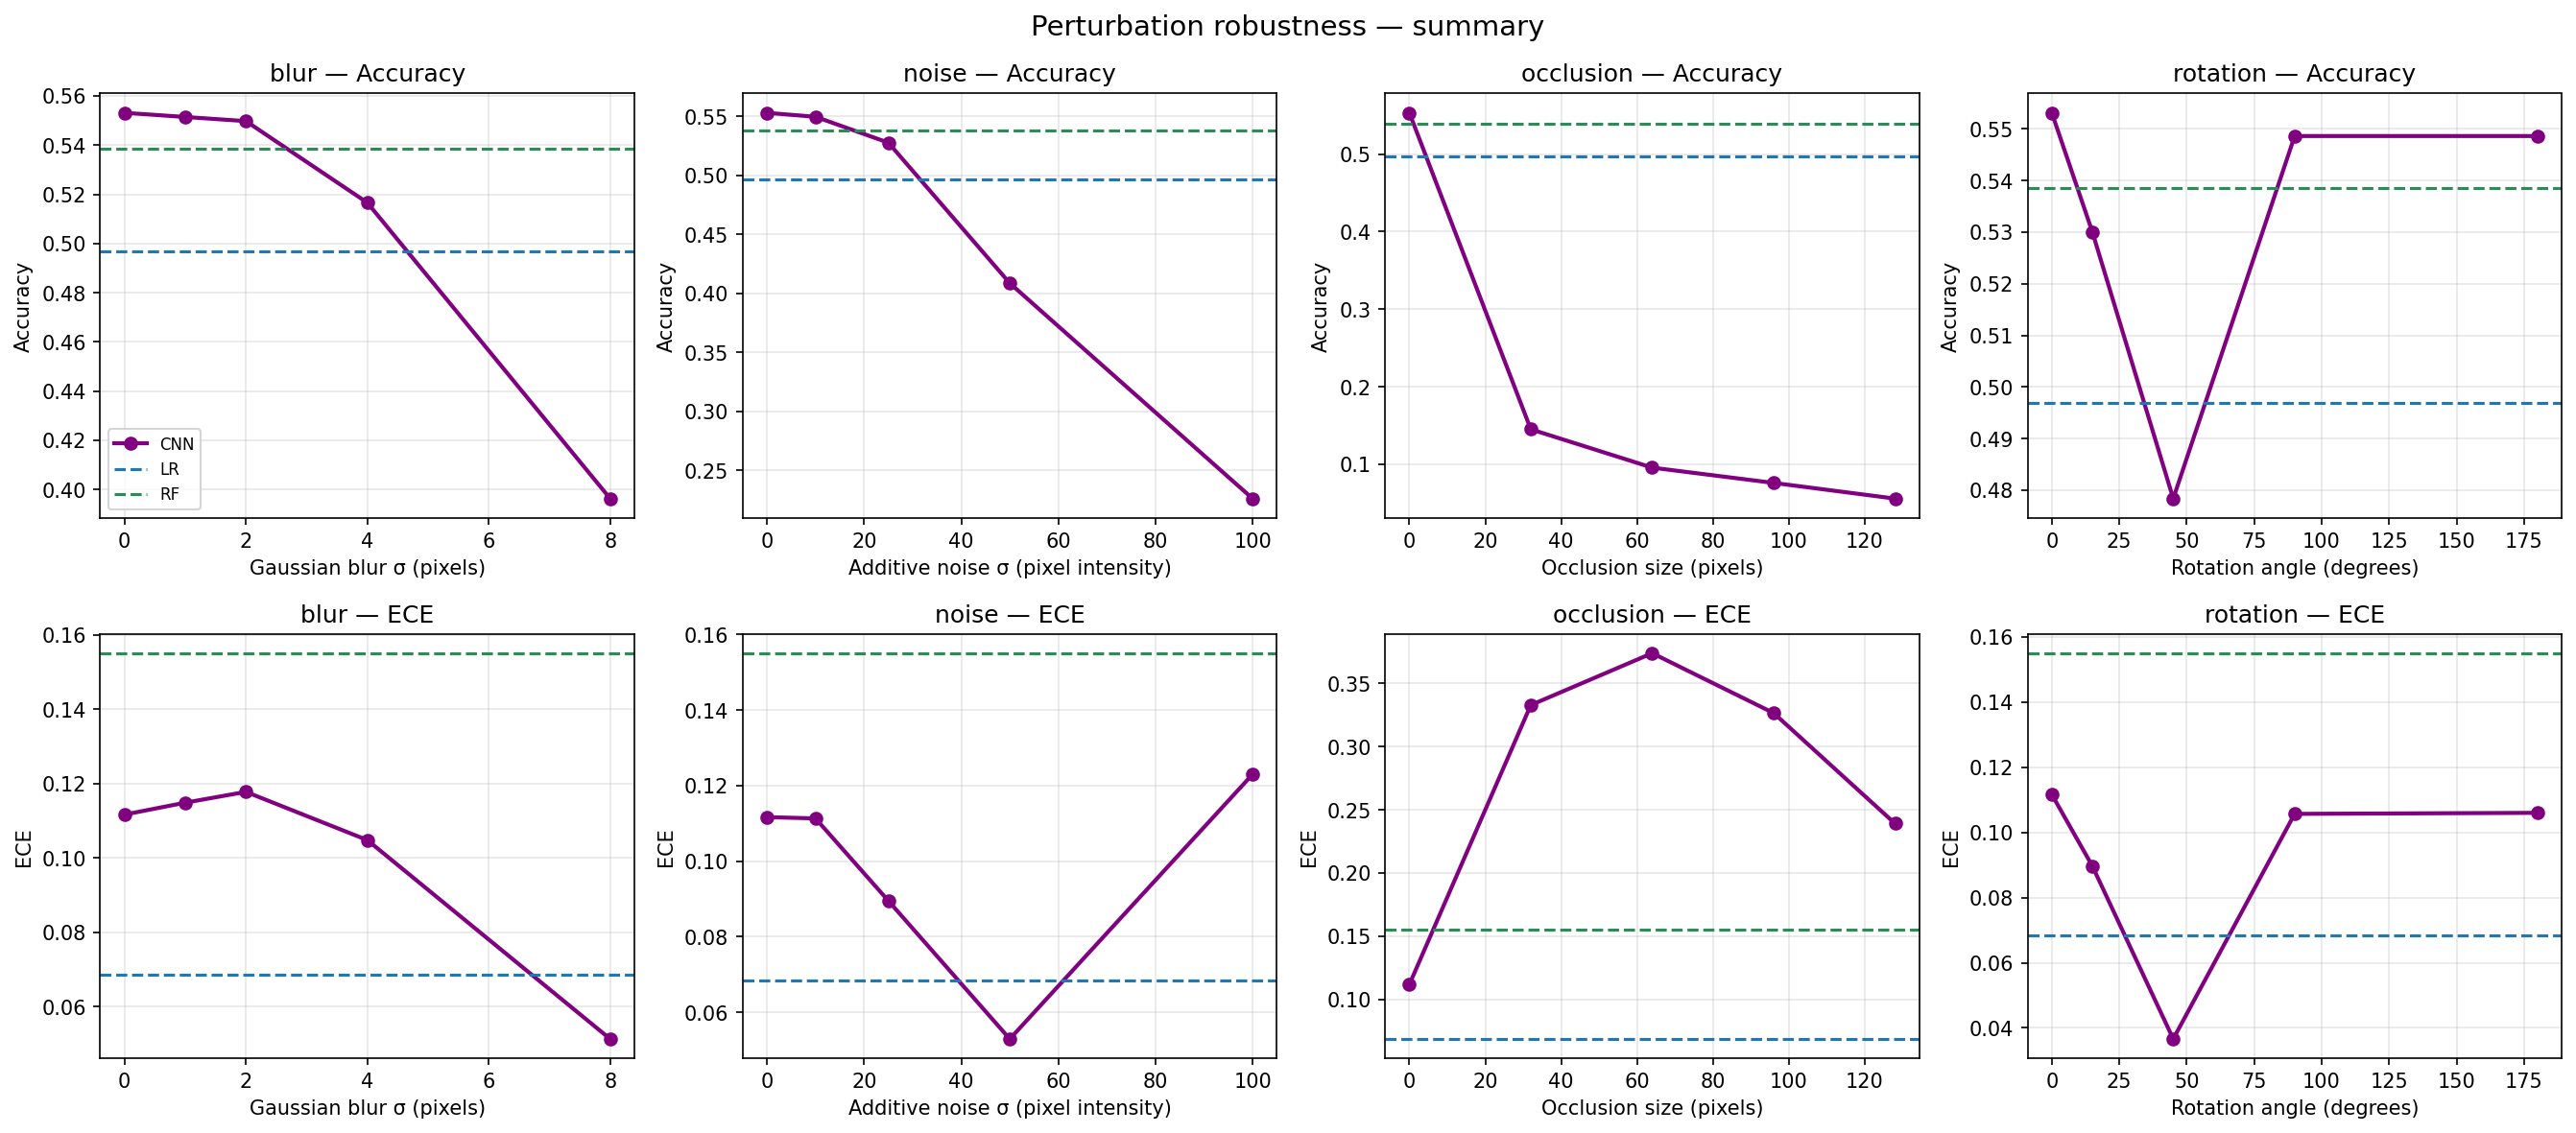
\includegraphics[width=\linewidth]{../results/figures/06_summary.png}
  \caption{Calibration vs.\ perturbation strength on a common $1{,}779$-sample hold-out (the headline plot).}
\end{subfigure}
\caption{(a) LR is closest to the diagonal, the CNN is over-confident in its top bin, RF is the worst. (b) At 50\% coverage on the CNN max-softmax the error rate is roughly halved. (c) ECE and accuracy vs.\ corruption strength for the four perturbation families; the panels show how each model degrades.}\label{fig:calib}
\end{figure}

\textbf{Clean-data ranking.} The CNN dominates on accuracy, F1 and NLL (Tab.~\ref{tab:agg}); LR has the lowest ECE despite the worst accuracy. Structurally, the convex L2 objective converges to the proper-scoring-rule optimum and the linear head cannot inflate confidence the way over-parameterised networks trained to convergence on NLL do \citep{guo2017}. The CNN's ECE is the visual average of two opposite failure modes (per-class numbers in \texttt{05g\_per\_class\_ece.json}): it is \emph{under-confident} on Round Smooth (per-class ECE 0.30, acc 0.86 vs.\ mean confidence 0.56) and \emph{over-confident} on a small Loose Spiral / Edge-on-w/Bulge top bin (top-bin gap $+0.94$ and $+0.78$ on 1 and 11 samples). Class-weighted training also pushes the minority Cigar class (n=334) toward conservative under-confidence (mean conf 0.49 vs.\ acc 0.72; per-class ECE 0.22, \emph{below} Round Smooth) -- the information-theoretically safer side of miscalibration. Cigar errors flow into Edge-on without/with Bulge in the confusion matrix.

\textbf{Robustness under perturbation (Fig.~\ref{fig:calib}c, Fig.~\ref{fig:perturb}).} Numbers in this paragraph come from the reduced perturbation-sweep CNN ($32\!\times\!32$, $M{=}2$, 5 epochs); absolute accuracies differ from the full ensemble (Tab.~\ref{tab:agg}) but the trend across corruption strength is the quantity of interest. The four corruption families fail in qualitatively different ways: (i) \textbf{rotation} barely affects the model -- the augmentation is exact at $\{0^\circ,90^\circ,180^\circ\}$ and the $15^\circ/45^\circ$ degradations are small ($<3$\,pp accuracy drop) -- expected from the equivariance baked in at training; (ii) \textbf{blur}: graceful degradation, accuracy $0.55\!\to\!0.40$ at $\sigma{=}8$, raw ECE actually decreases ($0.11\!\to\!0.05$) because the network correctly becomes less confident; (iii) \textbf{additive noise}: accuracy collapses sharply between $\sigma{=}25$ and $\sigma{=}50$ ($0.53\!\to\!0.41$) and ECE rises only once accuracy collapses; (iv) \textbf{occlusion} is catastrophic -- at $s{=}32$ accuracy drops to $0.15$ while ECE triples to $0.33$, and mean confidence on \emph{wrong} predictions \emph{rises} from 0.36 (clean) to 0.47 (occluded). The network is confidently wrong.

\textbf{Temperature scaling helps only on near shifts.} Fitting $T^\star$ on the clean holdout gives $T^\star{=}0.73{<}1$ (the model is under-confident, consistent with class-weighted ensembling) and cuts raw ECE from $0.11$ to $0.04$. Applying that same $T^\star$ keeps ECE around $0.03\text{--}0.04$ under blur and mild noise, but on occlusion at $s{=}32$ T-scaled ECE \emph{rises} to $0.43$ (vs.\ $0.33$ raw) and on heavy noise $\sigma{=}50$ it doubles to $0.12$. Sharpening a model that is already wrong moves it further from the diagonal -- the \citet{ovadia2019} mechanism.

\textbf{The ensemble does signal what it does not know.} Decomposing $H[\bar p]=\mathbb{E}[H[p_m]]+\big(H[\bar p]-\mathbb{E}[H[p_m]]\big)$ into aleatoric and epistemic parts: aleatoric stays in $1.2\text{--}1.7$ across all conditions; epistemic is flat under blur ($0.05\!\to\!0.08$) and rotation ($\approx\!0.05$) but rises $6{\times}$ under occlusion ($0.05\!\to\!0.32$) and $4{\times}$ under heavy noise ($0.05\!\to\!0.20$). So even when the mean-softmax is miscalibrated, the \emph{member disagreement} correctly flags the OOD-like shifts. Headline finding: \textbf{deep ensembles are well-calibrated under perturbations whose statistics are close to the augmentation distribution, and miscalibrated in mean-softmax but informative in member-disagreement under structurally different perturbations} \citep{lakshminarayanan2017,ovadia2019}.

\begin{figure}[h]
\centering
\begin{subfigure}{0.49\textwidth}
  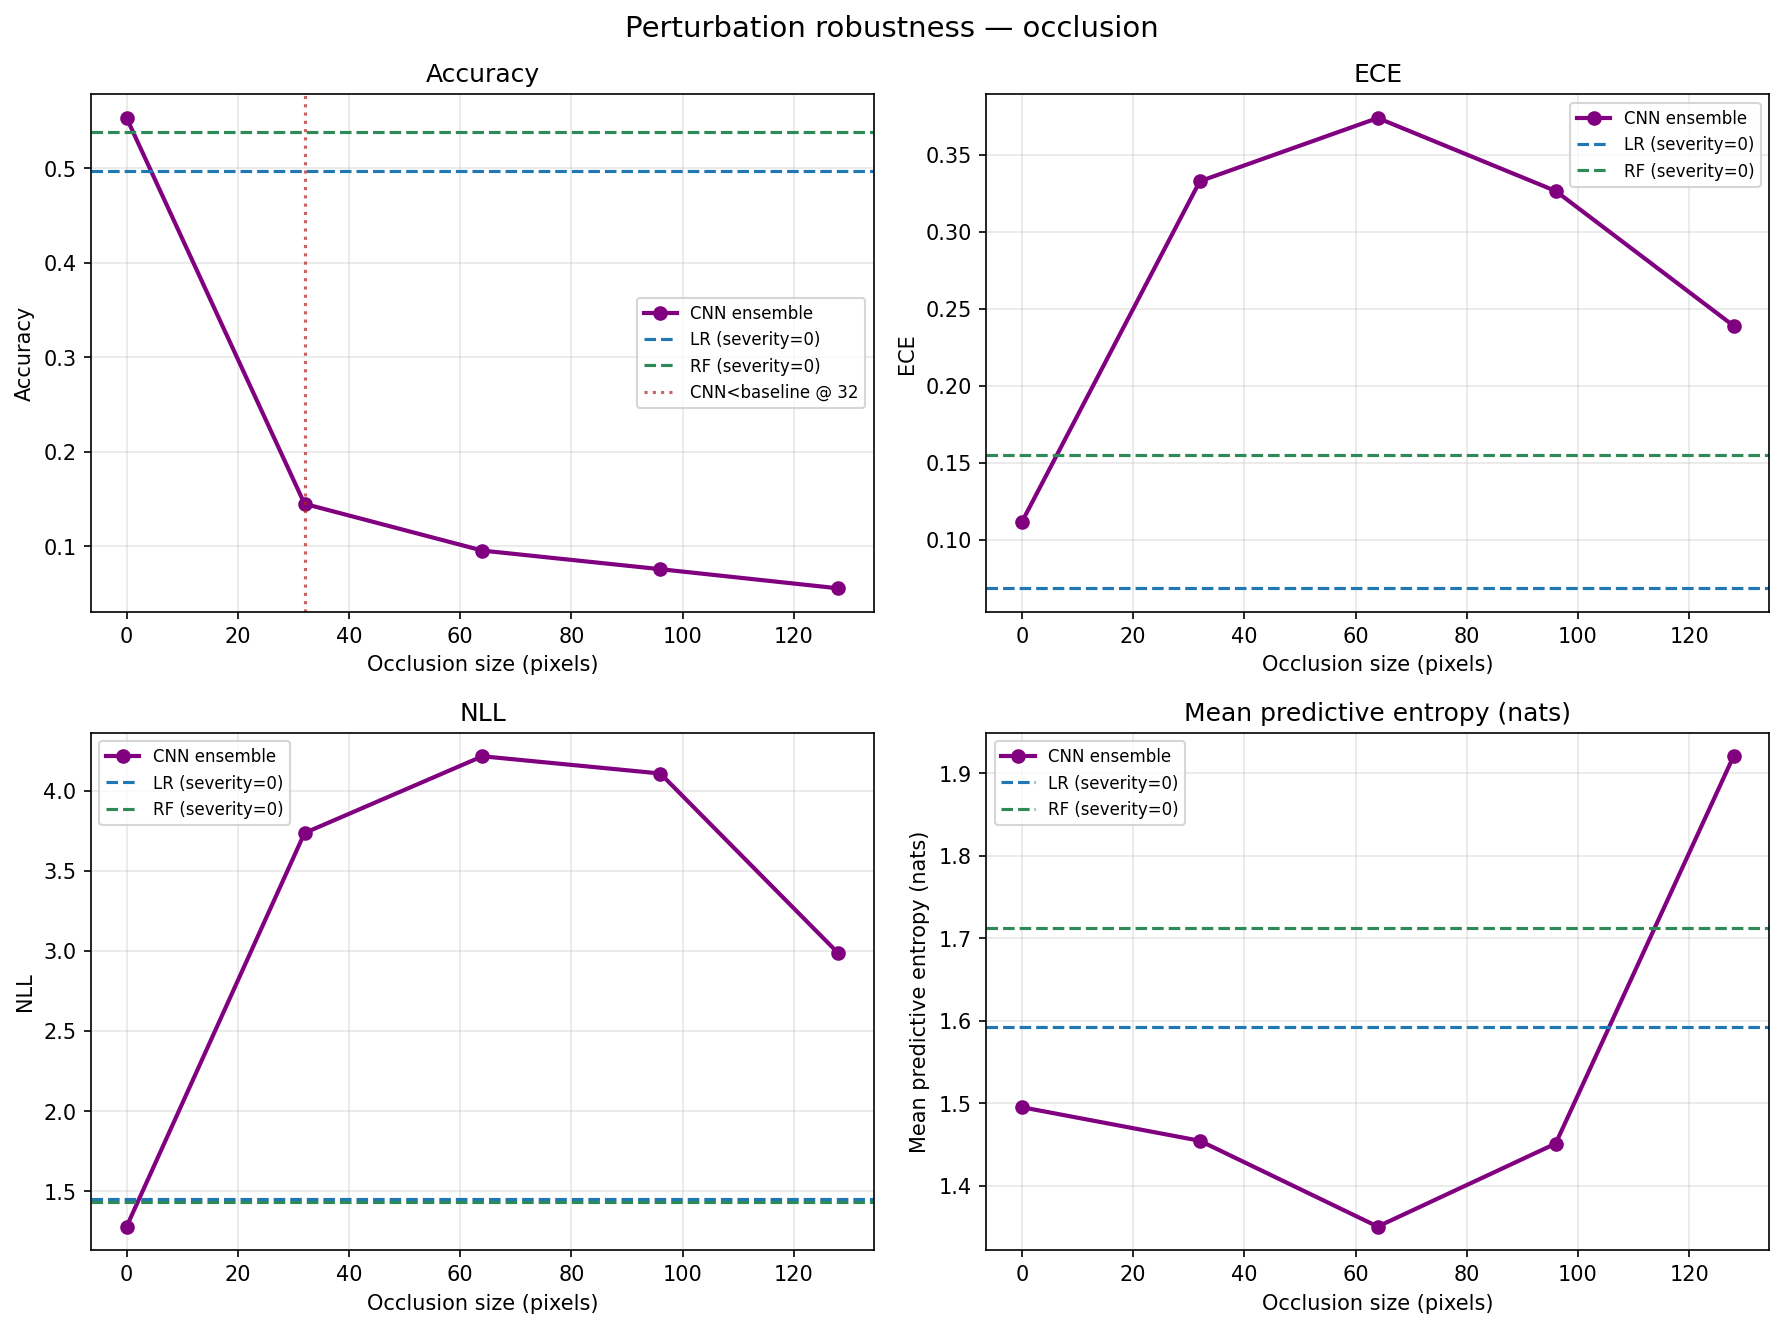
\includegraphics[width=\linewidth]{../results/figures/06_occlusion.png}
  \caption{Occlusion: ECE up, entropy low -- confidently wrong.}
\end{subfigure}\hfill
\begin{subfigure}{0.49\textwidth}
  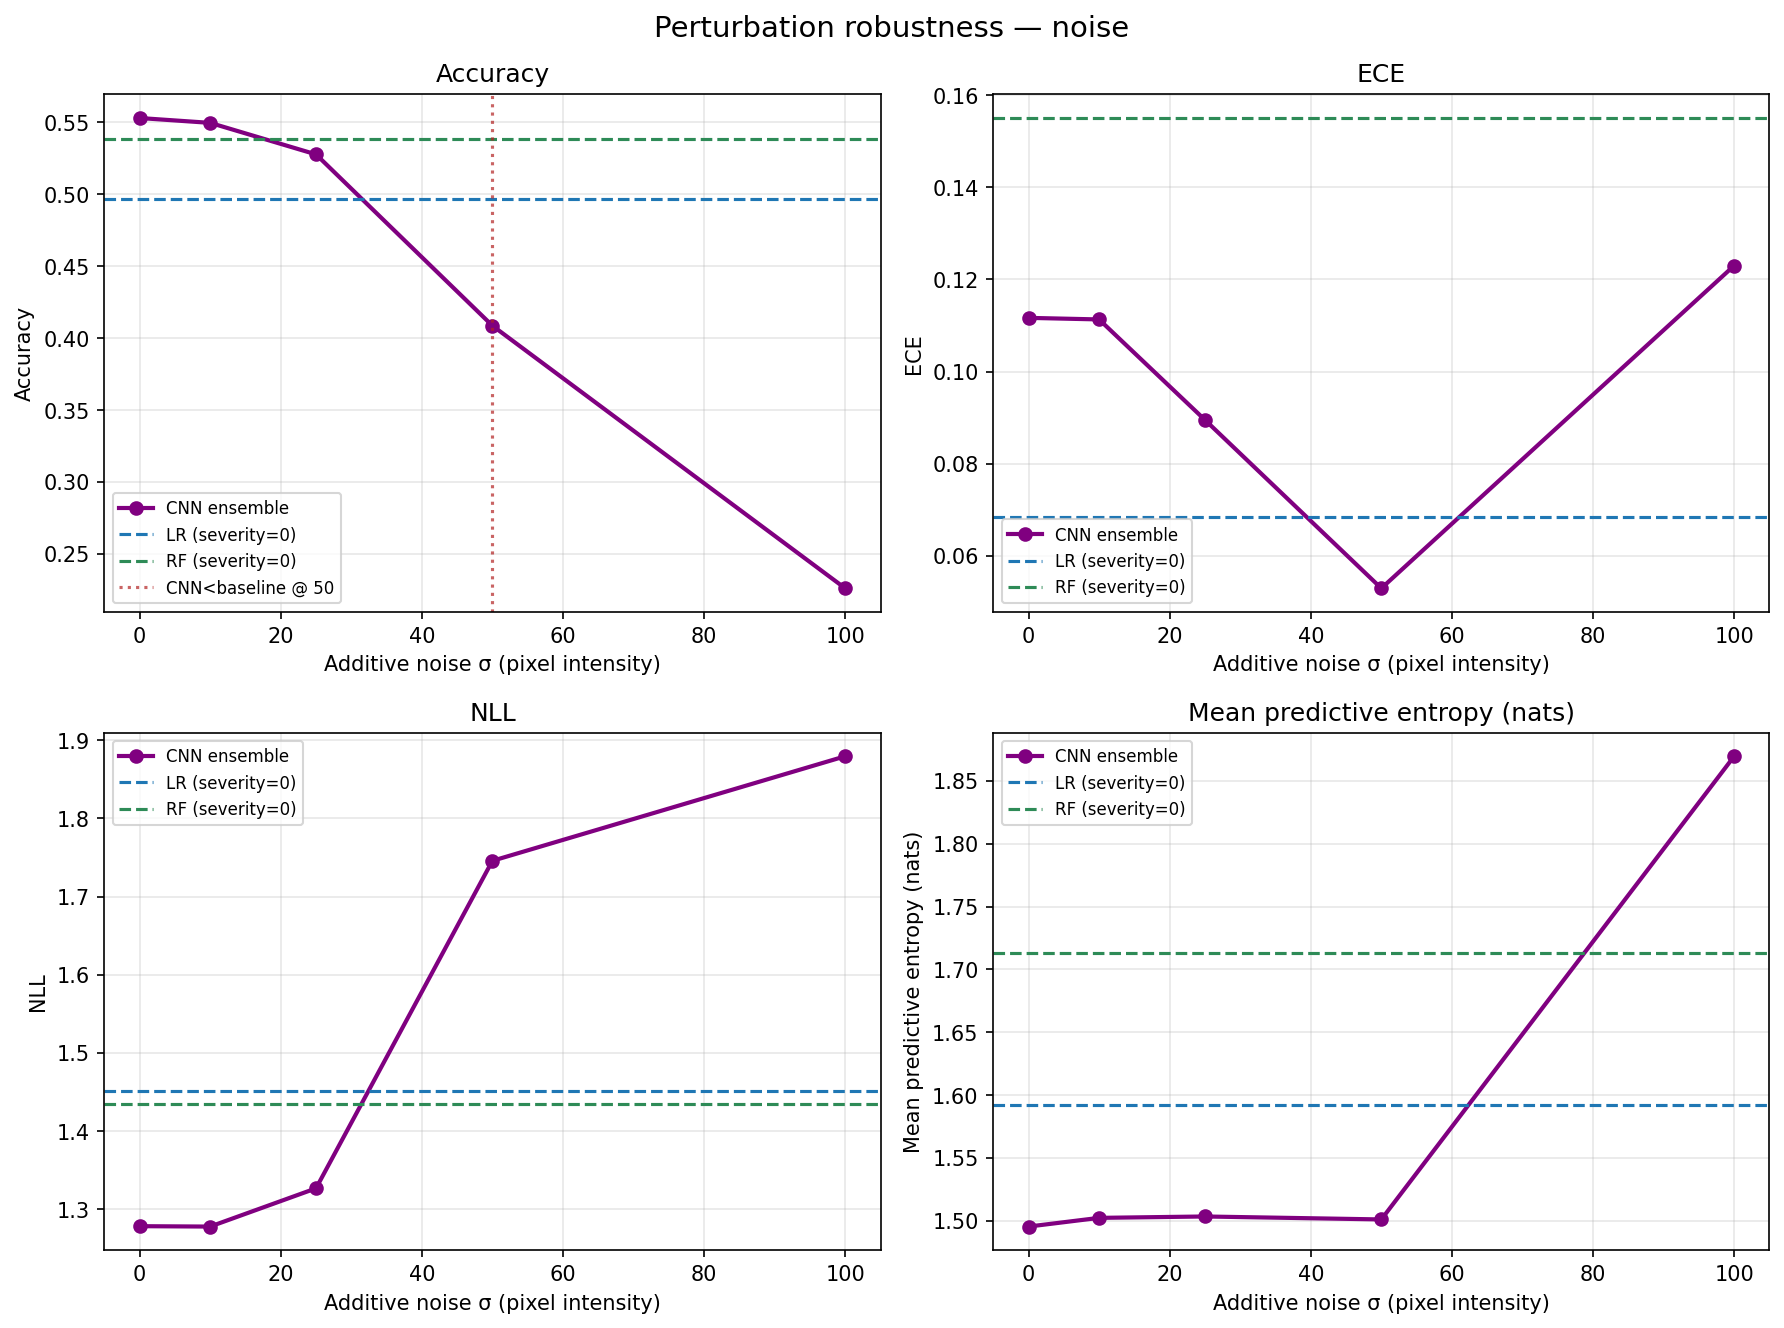
\includegraphics[width=\linewidth]{../results/figures/06_noise.png}
  \caption{Noise: accuracy drops, but predictive entropy correctly increases.}
\end{subfigure}
\caption{Per-perturbation breakdown of the two failure-mode extremes.}\label{fig:perturb}
\end{figure}

\textbf{Alternatives considered.} (a) Bootstrap CV: rejected, would leave some folds with zero Cigar samples. (b) Pretrained ResNet: would contaminate calibration claims with ImageNet statistics not present in our training distribution. (c) MC-Dropout instead of ensembles: equivalent in principle, but ensemble diversity comes from independent loss basins; on a 10-class imbalanced dataset the resulting member disagreement on minority-class samples is a stronger epistemic signal than dropout perturbations of a single optimum can produce \citep{lakshminarayanan2017}. (d) Selective prediction as a model variant: instead used post-hoc on every model's confidences (Fig.~\ref{fig:calib}b). (e) Temperature scaling as the calibration story: quantified above -- helps on near shifts, hurts on far shifts, so the case is for per-input mechanisms (ensemble disagreement) rather than scalar post-hoc fixes.

\textbf{Limitations.} (i) Perturbation sweep uses a smaller CNN ($32\!\times\!32$, $M{=}2$) than the headline ensemble; the trends and the epistemic-vs-aleatoric story are robust to scale, but absolute ECE numbers will be different for the full $M{=}5$, $64\!\times\!64$ ensemble. (ii) Sky-survey covariate shifts (different telescope, different filter set) are not simulated -- our corruptions are pixel-level, not instrument-level. (iii) Inner $k{=}3$ has visible variance in the inner macro-F1 ($\sim\!0.01$); a larger inner $k$ would tighten HP selection at non-trivial compute cost.

% -- Conclusion ----------------------------------------------------------------
\section{Conclusion}
We asked whether clean-data calibration rankings are preserved under shift. They are not: LR's clean-data calibration advantage over the CNN inverts under heavy occlusion, where the CNN becomes confidently wrong while LR's structurally lower confidence proves the more honest signal. Across three classifiers of increasing complexity, the deep ensemble CNN wins on accuracy, macro-F1 and NLL but is not the best-calibrated model on clean data -- a regularised logistic regression is. Under shift, rotation and blur degrade the CNN honestly, while occlusion and heavy noise produce confidently wrong predictions whose mean-softmax ECE more than triples; but the ensemble's \emph{member disagreement} rises sharply ($6{\times}$ epistemic entropy under heavy occlusion) precisely on those shifts, so the right uncertainty signal is in the spread, not in the mean. A single scalar temperature fit on clean data sharpens calibration on near-distribution corruptions and \emph{worsens} it on far-distribution ones, by construction. For a downstream pipeline consuming galaxy-classification probabilities, this argues for (i) deep ensembles over single networks, (ii) per-input thresholds on \emph{epistemic} entropy (not just max-softmax), and (iii) explicit OOD detectors tuned to occlusion-like corruptions, which post-hoc calibration alone cannot handle -- aligning with the broader findings of \citet{ovadia2019} on a different domain.

% -- Bibliography --------------------------------------------------------------
\renewcommand{\refname}{\vspace{-1.3em}}
\section*{Bibliography}
\footnotesize
\begin{thebibliography}{9}
\bibitem[Leung and Bovy(2019)]{leung2019} Leung, H. W., \& Bovy, J. (2019). Deep learning of multi-element abundances from high-resolution spectroscopic data. \textit{MNRAS}, 483(3), 3255--3277. Dataset: \url{https://astronn.readthedocs.io/en/latest/galaxy10.html}.
\bibitem[Lakshminarayanan et al.(2017)]{lakshminarayanan2017} Lakshminarayanan, B., Pritzel, A., \& Blundell, C. (2017). Simple and scalable predictive uncertainty estimation using deep ensembles. \textit{NeurIPS}.
\bibitem[Guo et al.(2017)]{guo2017} Guo, C., Pleiss, G., Sun, Y., \& Weinberger, K. Q. (2017). On calibration of modern neural networks. \textit{ICML}.
\bibitem[Ovadia et al.(2019)]{ovadia2019} Ovadia, Y., Fertig, E., Ren, J., Nado, Z., Sculley, D., Nowozin, S., Dillon, J., Lakshminarayanan, B., \& Snoek, J. (2019). Can you trust your model's uncertainty? Evaluating predictive uncertainty under dataset shift. \textit{NeurIPS}.
\bibitem[Hendrycks and Dietterich(2019)]{hendrycks2019} Hendrycks, D., \& Dietterich, T. (2019). Benchmarking neural network robustness to common corruptions and perturbations. \textit{ICLR}.
\bibitem[Lintott et al.(2008)]{lintott2008} Lintott, C., et al. (2008). Galaxy Zoo: Morphologies derived from visual inspection of galaxies from the SDSS. \textit{MNRAS}, 389(3), 1179--1189.
\bibitem[Dieleman et al.(2015)]{dieleman2015} Dieleman, S., Willett, K. W., \& Dambre, J. (2015). Rotation-invariant CNNs for galaxy morphology prediction. \textit{MNRAS}, 450(2), 1441--1459.
\bibitem[Conselice(2003)]{conselice2003} Conselice, C. J. (2003). The relationship between stellar light distributions of galaxies and their formation histories. \textit{ApJS}, 147(1), 1--28.
\bibitem[Lotz et al.(2004)]{lotz2004} Lotz, J. M., Primack, J., \& Madau, P. (2004). A new nonparametric approach to galaxy morphological classification. \textit{AJ}, 128(1), 163--182.
\end{thebibliography}

\end{document}
